\section{Efficiency Evaluation \& Simulations}
  \label{section:comparison}
  We offer here a cost and efficiency comparison of this work with
  LVPC~\cite{10.1007/978-3-030-65411-5_18} and Donner~\cite{donner}. We focus on
  these due to their exclusive support of
  virtual channels over any number of base channels. We remind that LVPC
  achieves this via recursion, while Donner
  because it is variadic (cf. Table~\ref{table:comparison-features}).

  We count the communication, storage and on-chain cost of a virtual
  channel in each protocol. We also simulate the execution of a large number
  of payments among many parties and derive payment latency and fees. We thus
  obtain an end-to-end understanding of both the requirements and benefits
  of each protocol.

  \makeatletter%
  \@ifclassloaded{IEEEtran}%
    {\paragraph{Cost calculation}}%
    {\paragraph{Cost calculation.}}%
  \makeatother%
  Consider the setting of $1$
  funder ($P_1$), $1$ fundee ($P_n$) and $n-2$ intermediaries ($P_2, \dots,
  P_{n-1}$) where $P_i$ has a base channel with each of $P_{i-1}$,
  $P_{i+1}$. We compare the costs of off-chain opening
  (Table~\ref{table:comparison:overhead:n-parties:open}) and on-chain
  closing unilaterally
  (Table~\ref{table:comparison:overhead:n-parties:close}).
  See Appx.~\ref{section:cost-details} for comparison details and choices.

  Regarding opening, in
  Table~\ref{table:comparison:overhead:n-parties:open} we measure for each of
  the $3$ protocols the number of communication rounds required, the total
  size of outgoing messages as well as the amount of space for storing
  channel data. We measure funder, fundee
  and intermediary requirements, along with the aggregate for all parties.

  Regarding closing, % TODO: remove line to shorten
  in Table~\ref{table:comparison:overhead:n-parties:close} we
  measure for each of the three protocols the worst-case on-chain cost for a party
  in order to unilaterally close its channel. The cost is
  measured both in the number of transactions and in their total size.

  For the two endpoints (funder and fundee), we show the cost of unilaterally
  closing the virtual channel, whereas for each intermediary we
  report the cost of closing a base channel. We also present the worst-case
  total on-chain cost,
  aggregated over all parties. Note that the latter cost is not simply the sum
  of the worst-case costs of all parties, as one party's worst case is not
  necessarily the worst case of another. This cost rather represents the maximum
  possible load an instantiation of each protocol could add to the blockchain
  when closing.

  % TODO: understand why number of payments k plays a role in Donner
  % splncs
  \addtolength{\intextsep}{-21pt}
  \begin{table*}[h!]
    \resizebox{\textwidth}{!}{%
    \begin{tabular}{|l|c|c|c|c|c|c|c|c|c|c|c|}
    \hline
    \multicolumn{12}{|c|}{Open} \\
    \hline
    \multirow{3}{*}{}
              & \multicolumn{3}{|c|}{Funder} & \multicolumn{3}{|c|}{Fundee}
              & \multicolumn{3}{|c|}{Intermediary}
              & \multicolumn{2}{|c|}{Total} \\
    \cline{2-12}
              & \multirow{2}{*}{\shortstack{party \\ rounds}}
              & \multicolumn{2}{|c|}{size} & \multirow{2}{*}{\shortstack{party
              \\ rounds}} & \multicolumn{2}{|c|}{size}
              & \multirow{2}{*}{\shortstack{party \\ rounds}}
              & \multicolumn{2}{|c|}{size} & \multicolumn{2}{|c|}{size} \\
    \cline{3-4} \cline{6-7} \cline{9-12}
              & & sent & stored & & sent & stored & & sent & stored & sent &
              stored \\
    \hline
    LVPC      & $8(n-2)$ & $1381(n-2)$ & $3005(n-2)$ & $7$ & $1254$ & $2936$
              & $16$ & $2989$ & $6385$ & $4370n-8740$ & $9390n-18780$ \\
    \hline
    % my count
    %Donner     & $2$ & $164n + 1934$ & $108n + 2150$ & $1$ & $44n+128$
    %           & $176n+496$ & $1$ & $76n + 2010$ & $132n+2370$
    %           & $132n^2+2390n-2094$ & $76n^2+2066n-1858$ \\
    %\hline
    \multirow{2}{*}{Donner}
              & \multirow{2}{*}{$2$} & \multirow{2}{*}{$184n + 829$}
              & \multirow{2}{*}{\shortstack{$1332.5k+$ \\ $43n+125.5$}}
              & \multirow{2}{*}{$1$} & \multirow{2}{*}{$43n+192.5$}
              & \multirow{2}{*}{\shortstack{$1332.5k+$ \\ $43n+125.5$}}
              & \multirow{2}{*}{$1$} & \multirow{2}{*}{$547$}
              & \multirow{2}{*}{\shortstack{$1332.5k+$ \\ $43n+125.5$}}
              & \multirow{2}{*}{$774n-71$}
              & \multirow{2}{*}{\shortstack{$1332.5kn +$ \\ $43n^2 + 125.5n$}}
              \\
              & & & & & & & & & & & \\
              % For Donner, I drew the storage numbers from
              % https://eprint.iacr.org/2021/855.pdf, p. 22. I'm not sure what
              % pid is, so these numbers may have to be revised.
    \hline
    \multirow{3}{*}{Elmo}
              & \multirow{3}{*}{$6$} &
              \multirow{3}{*}{\shortstack{$32n^3-128n^2$ \\
              $+544n-276$}} &
              \multirow{3}{*}{\shortstack{$\frac{128}{3}n^3-128n^2$ \\
              $+\frac{1276}{3}n+220$}} &
              \multirow{3}{*}{$6$}
              & \multirow{3}{*}{\shortstack{$32n^3-128n^2$ \\
              $+544n-340$}} &
              \multirow{3}{*}{\shortstack{$\frac{128}{3}n^3-128n^2$ \\
              $+\frac{1276}{3}n+220$}} &
              \multirow{3}{*}{$12$}
              & \multirow{3}{*}{\shortstack{$96n^3-256n^2$ \\
              $+404n-40$}}
              & \multirow{3}{*}{\shortstack{$96n^3-256n^2$ \\
              $+468n+88$}}
              & \multirow{3}{*}{\shortstack{$96n^4-384n^3+$ \\
              $724n^2+240n-792$}} &
              \multirow{3}{*}{\shortstack{$96n^4-\frac{1088}{3}n^3+$ \\
              $660n^2+\frac{8}{3}n+520$}}\\
              & & & & & & & & & & & \\
              & & & & & & & & & & & \\
    \hline
    \end{tabular}}
    \caption{Open efficiency comparison of virtual channel protocols with $n$
    parties and $k$ payments.}
    \label{table:comparison:overhead:n-parties:open}
  \end{table*}
  % splncs
  \addtolength{\intextsep}{21pt}

  % splncs
  \addtolength{\intextsep}{-25pt}
  \begin{table*}[h!]
    \begin{minipage}{\textwidth}
    \centering
    \begin{tabular}{|l|c|c|c|c|c|c|c|c|}
    \hline
    \multicolumn{9}{|c|}{Unilateral Close} \\
    \hline
              & \multicolumn{2}{|c|}{Intermediary}
              & \multicolumn{2}{|c|}{Funder} & \multicolumn{2}{|c|}{Fundee}
              & \multicolumn{2}{|c|}{Total} \\
    \hline
              & \#txs & size & \#txs & size & \#txs & size & \#txs & size \\
    \hline
    LVPC      & $3$ & $627$ & $2$ & $383$ & $2$ & $359$ & $2n-2$ & $435n -
              510.5$ \\
    \hline
    Donner    & $1$ & $204.5$ & $4$ & $704 + 43n$ & $1$ & $136.5$ & $2n$ & $458n
              - 26$ \\
    \hline
    Elmo      & $1$ & $297.5$ & $3$ & $376$ & $3$ & $376$
              & $n+1$ & $254.5n-133$ \\
    \hline
    \end{tabular}
    \end{minipage}
    \caption{On-chain worst-case closing efficiency comparison of virtual
    channel protocols with $n$ parties.}
    \label{table:comparison:overhead:n-parties:close}
  \end{table*}
  % splncs
  \addtolength{\intextsep}{25pt}

  We note that Elmo exploits
  MuSig2~\cite{DBLP:journals/dcc/MaxwellPSW19,DBLP:conf/crypto/NickRS21} to
  reduce both its
  on-chain and storage footprint: the $n$ signatures that are needed to spend
  each virtual and bridge output can be securely reduced to a single aggregate
  signature. The same cannot be said for
  Donner, since this technique cannot optimise away the $n$ outputs of the
  funder's transaction $\tx^{\mathtt{vc}}$. Likewise LVPC cannot gain a linear
  improvement with this optimisation, since each of its relevant transactions
  (``split'', ``merge'' and ``refund'') needs constant signatures.

  We furthermore note that, since human connections form a
  small world~\cite{smallworld}, we expect that in practice the
  need for virtual channels with a large number of
  intermediaries will be exceedingly rare. This is corroborated by
  the fact that LN only supports payments of up to $20$ hops
  without impact to its usefulness. Therefore, the asymptotic
  network and storage complexity are not as relevant as the
  concrete costs for specific, low values of $n$. Under this
  light, the overhead of Elmo is tolerable. For example, the
  total size of messages sent and received for a funder when opening an Elmo channel
  of length $n=6$ are less than $3$ times those of Donner and
  slightly cheaper than LVPC
  (Table~\ref{table:comparison:overhead:n-parties:open}).

  \makeatletter%
  \@ifclassloaded{IEEEtran}%
    {\paragraph{Payment simulations}}%
    {\paragraph{Payment simulations.}}%
  \makeatother%
  We implemented a simulation
  framework\footnote{\url{gitlab.com/anonymised-submission-8778e084/virtual-channels-simulation}}
  in which a list of randomly generated payments are carried out.
  A single simulation is parametrised by a list of payments
  (sender, receiver, value triples), the protocol (Elmo, Donner, LVPC, LN or
  on-chain only), which future payments each payer knows and the utility
  function it maximises. The knowledge function defines which future payments
  inform each decision.
  Our simulation framework is of independent interest, as it is flexible
  and reusable for a variety of payment network protocol evaluations.

  We here
  show the performance of the $3$ protocols with respect to the metrics payment
  channels aim to improve, namely payment latency (Fig.~\ref{graph:delays}) and
  fees (Fig.~\ref{graph:fees}). We have designed 3 workloads: ``power law'', in
  which incoming payments follow a zipf~\cite{powers-1998-applications}
  distribution, ``preferred receiver'', in which each party has a preferred
  payee which receives half of the payments, and ``uniform'', where payments are
  chosen uniformly at random. See Appx.~\ref{section:simulation-details} for
  more details.

  As evidenced, Elmo is the best or on par with the best protocol in every
  case. We attribute this to the flexibility of Elmo, as it is both variadic and
  recursive, thus able to exploit the cheapest payment method in all scenarios.
  In particular, Donner is consistently the most fee-heavy protocol and LVPC the
  slowest. Elmo experiences similar delays to Donner and slightly higher fees
  than LVPC.

  % TODO: consider converting figures into tables
  % splncs
  \addtolength{\intextsep}{-15pt}
  \begin{figure*}
  \begin{subfigure}{.3293\textwidth}
  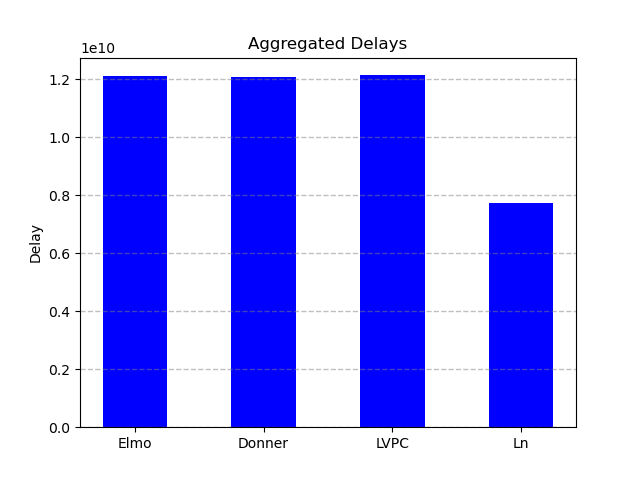
\includegraphics[width=\textwidth]{../simulation/Delays_power_law.png}
  \end{subfigure}
  \begin{subfigure}{.3293\textwidth}
  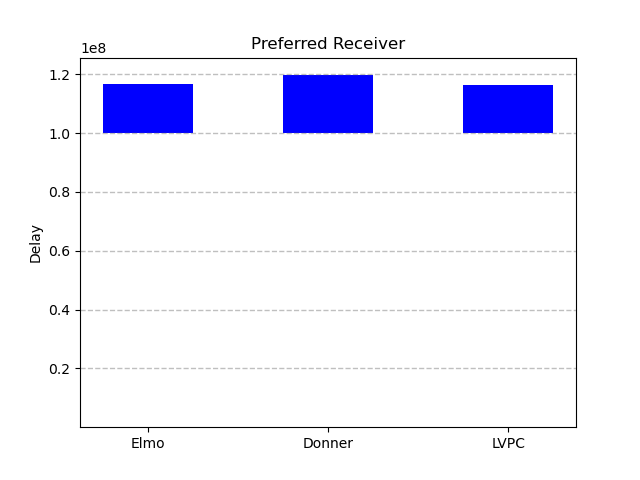
\includegraphics[width=\textwidth]{../simulation/Delays_preferred_receiver.png}
  \end{subfigure}
  \begin{subfigure}{.3293\textwidth}
  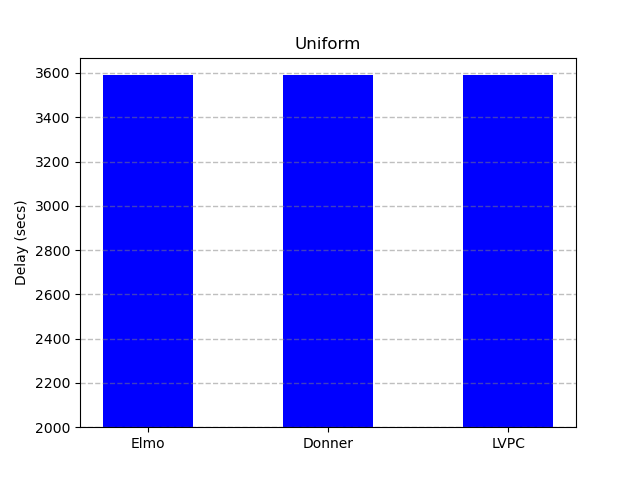
\includegraphics[width=\textwidth]{../simulation/Delays_uniform.png}
  \end{subfigure}
  \caption{Average per-payment delay (both on- and off-chain) in
  sec. Less is better.}
  \label{graph:delays}
  \end{figure*}
  \begin{figure*}
  \begin{subfigure}{.3293\textwidth}
  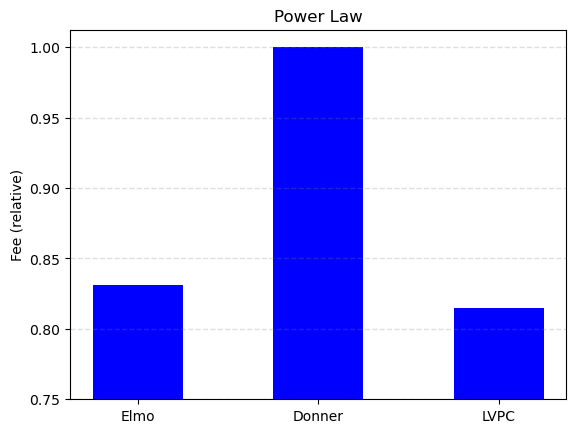
\includegraphics[width=\textwidth]{../simulation/Fees_power_law.png}
  \end{subfigure}
  \begin{subfigure}{.3293\textwidth}
  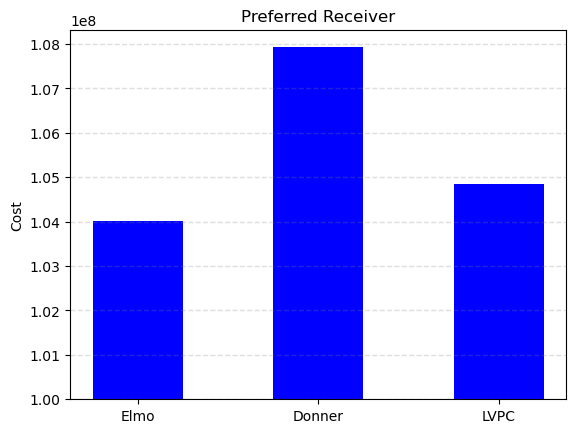
\includegraphics[width=\textwidth]{../simulation/Fees_preferred_receiver.png}
  \end{subfigure}
  \begin{subfigure}{.3293\textwidth}
  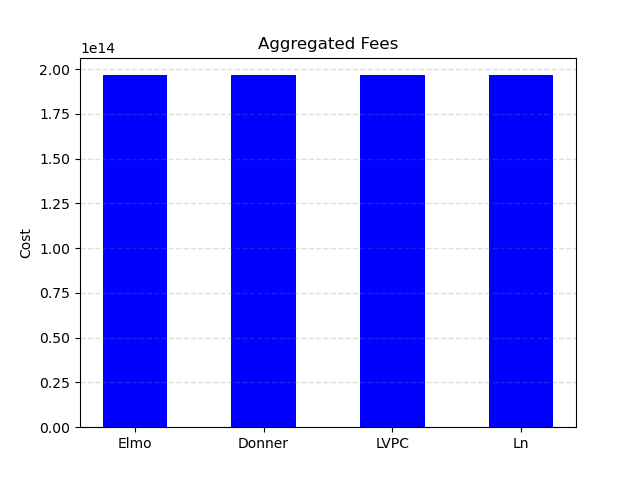
\includegraphics[width=\textwidth]{../simulation/Fees_uniform.png}
  \end{subfigure}
  \caption{Average per-payment relative fee. Less is better.}
  \label{graph:fees}
  \end{figure*}
  % splncs
  \addtolength{\intextsep}{15pt}
